%%%%%%%%%%%%%%%%%%%%%%%%%%%%%%%%%%%%%%%%%
% Journal Article
% LaTeX Template
% Version 1.4 (15/5/16)
%
% This template has been downloaded from:
% http://www.LaTeXTemplates.com
%
% Original author:
% Frits Wenneker (http://www.howtotex.com) with extensive modifications by
% Vel (vel@LaTeXTemplates.com)
%
% License:
% CC BY-NC-SA 3.0 (http://creativecommons.org/licenses/by-nc-sa/3.0/)
%%%%%%%%%%%%%%%%%%%%%%%%%%%%%%%%%%%%%%%%%

%----------------------------------------------------------------------------------------
%	PACKAGES AND OTHER DOCUMENT CONFIGURATIONS
%----------------------------------------------------------------------------------------

\documentclass[twoside,twocolumn]{article}

\usepackage{blindtext} % Package to generate dummy text throughout this template

\usepackage[sc]{mathpazo} % Use the Palatino font
\usepackage[T1]{fontenc} % Use 8-bit encoding that has 256 glyphs
\linespread{1.05} % Line spacing - Palatino needs more space between lines
\usepackage{microtype} % Slightly tweak font spacing for aesthetics

\usepackage[german]{babel} % Language hyphenation and typographical rules

\usepackage[hmarginratio=1:1,top=32mm,columnsep=20pt]{geometry} % Document margins
\usepackage[hang, small,labelfont=bf,up,textfont=it,up]{caption} % Custom captions under/above floats in tables or figures
\usepackage{booktabs} % Horizontal rules in tables

\usepackage{lettrine} % The lettrine is the first enlarged letter at the beginning of the text

\usepackage{enumitem} % Customized lists
\setlist[itemize]{noitemsep} % Make itemize lists more compact

\usepackage{abstract} % Allows abstract customization
\renewcommand{\abstractnamefont}{\normalfont\bfseries} % Set the "Abstract" text to bold
\renewcommand{\abstracttextfont}{\normalfont\small\itshape} % Set the abstract itself to small italic text

\usepackage{titlesec} % Allows customization of titles
\renewcommand\thesection{\Roman{section}} % Roman numerals for the sections
\renewcommand\thesubsection{\roman{subsection}} % roman numerals for subsections
\titleformat{\section}[block]{\large\scshape\centering}{\thesection.}{1em}{} % Change the look of the section titles
\titleformat{\subsection}[block]{\large}{\thesubsection.}{1em}{} % Change the look of the section titles

\usepackage{fancyhdr} % Headers and footers
\pagestyle{fancy} % All pages have headers and footers
\fancyhead{} % Blank out the default header
\fancyfoot{} % Blank out the default footer
\fancyhead[C]{Evolutionäre Optimierungsalgorithmen $\bullet$ MK - Einführung in das wissenschaftliche Arbeiten} % Custom header text
\fancyfoot[RO,LE]{\thepage} % Custom footer text

\usepackage{titling} % Customizing the title section

\usepackage{hyperref} % For hyperlinks in the PDF

\newcommand{\e}[1]{\times 10^{#1}}

\usepackage{graphicx}

\usepackage{amsmath}

%----------------------------------------------------------------------------------------
%	TITLE SECTION
%----------------------------------------------------------------------------------------

\setlength{\droptitle}{-4\baselineskip} % Move the title up

\pretitle{\begin{center}\Huge\bfseries} % Article title formatting
\posttitle{\end{center}} % Article title closing formatting
\title{Evolutionäre Optimierungsalgorithmen} % Article title
\author{
	\textsc{Federico Ramírez Villagrana} \\[1ex]
	\normalsize Universität Hamburg \\
	\normalsize Methodenkompetenz - Einführung in das wissenschaftliche Arbeiten \\
	\normalsize Dozent: Dr. Andreas Günther
}
\date{} % Leave empty to omit a date
\renewcommand{\maketitlehookd}{%
\begin{abstract}
\noindent In diesem Paper wird es darüber diskutiert, sowohl was Optimierung ist und warum ist es schwer, als auch was evolutionärer Algorithmen (EA) sind und wie, warum,  und wann sind sie hilfreich in dem Optimierung-Bereich. Es wird auch im Detail erklärt, wie EA funktionieren und warum sind sie als teil des künstlichen Intelligenz (KI) betrachtet. Es werden auch einige bekannten EA präsentiert und leicht erklärt. Am ende wird es darüber diskutiert, was für Vor- und Nachteile die EA haben.
\end{abstract}
}

%----------------------------------------------------------------------------------------

\begin{document}

% Print the title
\maketitle

%----------------------------------------------------------------------------------------
%	ARTICLE CONTENTS
%----------------------------------------------------------------------------------------

\section{Einleitung}

\lettrine[nindent=0em,lines=3]{D} as Problem des Handlungsreisenden (engl. traveling salesman problem oder TSP) ist ein sehr bekanntes und studierte Problem in dem Informatik-Bereich und es geht wie folgendes:\\
Es muss eine Reihenfolge für den Besuch mehrerer Orte so gewählt sein, dass keine Station außer der ersten mehr als einmal besucht wird, die gesamte Reisestrecke des Handlungsreisenden möglichst kurz, und die erste Station gleich der letzten Station ist. \cite{wiki_tsp}\\
Sei $n$ die Anzahl der Stationen, es gibt $(n-1)!$ mögliche Lösungen für das TSP. Das heißt, dass für $n=4$ es gibt $6$ mögliche Lösungen. Es ist nicht schwer einen brute-force Ansatz zu verfolgen für ein Problem, das nur 6 Lösungen hat. Aber wenn $n=50$ es gibt circa $6,1\e{62}$ Lösungen! Folgendes ist hilfreich, um diese Anzahl in eine Perspektive zu setzen: Das Universum ist circa 15 Milliarde Jahre alt, das ist $4,7\e{17}$ Sekunden. Wenn es eine Billion Rechner gäbe, die jeder einzeln seit dem Anfang des Universums eine Billion Lösungen pro Sekunde berechnete. Bisher wären nur $4,7\e{41}$ Lösungen berechnet worden.\\
Das TSP ist nur ein Beispiel von vielfältigen Probleme, die zu den kombinatorischen Problemen gehören, das heißt, Probleme für die einfach keine brute-force Ansatz möglich ist. Es ist in diesem Fall, dass evolutionärer Algorithmen (EA) hilfreich sind.\\
EA sind eine gute Werkzeug um gute Lösungen zu finden. Natürlich können wir nicht sicher sein, dass wir das beste Lösung gefunden haben, außer wenn wir jeder mögliche Lösungen berechnen haben. Aber wie es mit obenen Beispiel gezeigt ist, es ist nicht immer möglich alle mögliche Lösungen zu finden.

%------------------------------------------------

\section{Stand der Forschung}

\lettrine[nindent=0em,lines=3]{L} orem ipsum dolor sit amet, consectetur adipiscing elit.
\blindtext % Dummy text

%------------------------------------------------

\section{Optimierung}

\lettrine[nindent=0em,lines=3]{I} n dem Mathematik-Bereich, Optimierung bedeutet die Findung von Parametern eines Systems, die ein bestmögliches Ergebnis erzielen. \cite{wiki_optimierung} Wir können diese Findung von Parametern auch wie Folgendes definieren: Die Auswahl von die bestmögliche Lösung eines Problems von einer Menge mögliche Lösungen.\\
In Optimierungsprobleme wird eine Zielfunktion (engl. objective function) definiert, die entweder maximiert oder minimiert werden soll. Die Zielfunktion wird ``Kosten-Funktion'' oder ``Fitness-Funktion'' in Maximierung- und Minimierungsprobleme bzw. genannt.\\
Sei $f(x)$ ein Zielfunktion, $x$ ist ein Vektor und wird Entscheidungsvariable genannt. Die Anzahl von Elementen in $x$ wird die Dimension des Problems genannt.\\
Es gibt verschiedene Klassifizierungen oder Arten von Optimierung:

\begin{itemize}
\item{Eingeschränkt Optimierung}\\
Die Entscheidungsvariable kann nicht irgendwelcher Wert nehmen. Es gibt Einschränkungen dafür.\\
\item{Multi-objective Optimierung}\\
Das Problem besteht aus vielfältigen, voneinander unabhängig Zielfunktionen.\\
\item{Multi-modal Optimierung}\\
Die Zielfunktion(en) hat/haben mehrere Minima bzw. Maxima. Abbildung \ref{fig:rastrigin} zeigt eine multi-modale Funktion.
\end{itemize}

\begin{figure}[h]
\caption{ Rastrigin function.}
\label{fig:rastrigin}
\centering
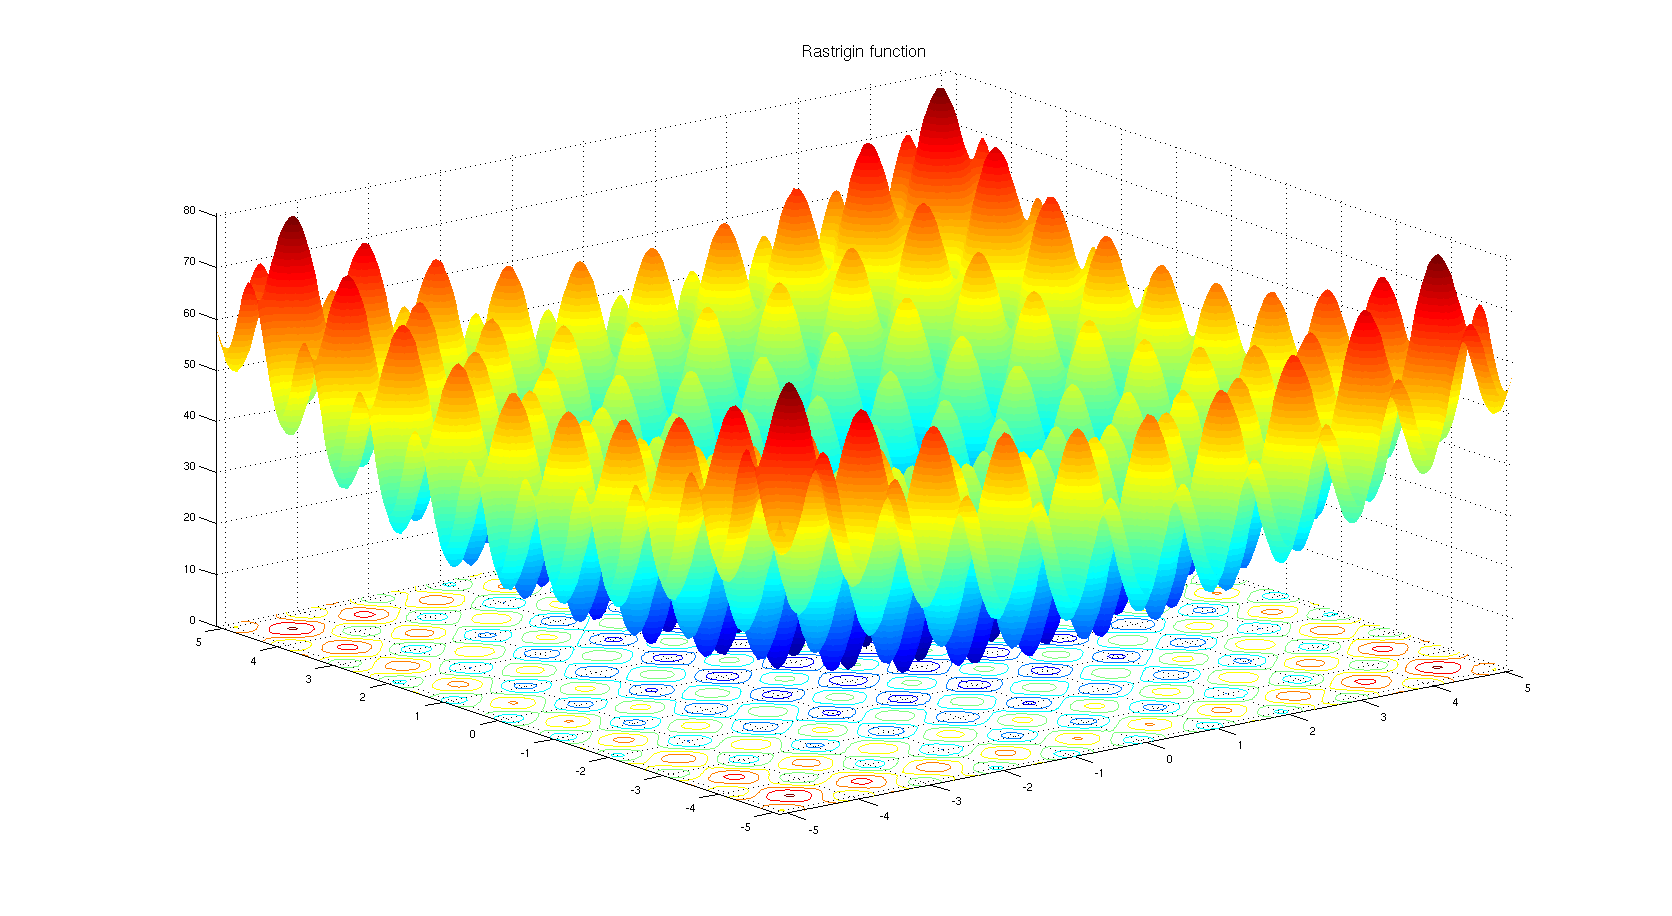
\includegraphics[width=0.5\textwidth]{images/rastrigin_function.png}
\end{figure}

Eine der wichtigste und schwersten Teile der Optimierung ist es, eine geeignete Zielfunktion zu definieren, die alle die wichtige zu optimieren Faktore berücksichtigt.
Probleme im wirklichen Leben sind normalerweise eingeschränkt, multi-Objective und multi-modale, oder mit eine hoch Anzahl von Dimensionen. Wegen diesen Eigenschaften der Zielfunktionen und der Optimierungsprobleme ist es schwer eine gute Lösung mittels traditionelle Vorgänge  zu finden. EA sind aber eine gute Möglichkeit, um diese Art von Probleme zu lösen.

%------------------------------------------------

\section{Was ist ein evolutionärer Algorithmus?}

\lettrine[nindent=0em,lines=3]{D} er EA-Bereich ist ziemlich neu, deswegen gibt es bisher keine allgemein akzeptierte Definition von evolutionäre Algorithmus. EA sind zwar als teil des KIs betrachtet, aber genau wo sie in Verbindung mit anderen KI-Methoden stehen ist von dem Autor abhängig. Abbildung \ref{fig:metaheuristics} zeigt eine von mehrere mögliche Klassifikationen von KI-Methoden in Bezug auf Metaheuristics (welche über den Rahmen dieses Papiers hinausgehen).\\

\begin{figure}[h]
\caption{ Klassifikation von Metaheuristics.}
\label{fig:metaheuristics}
\centering
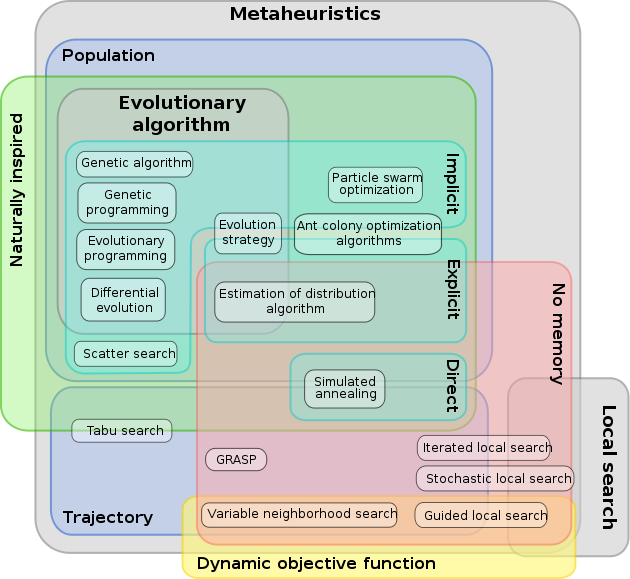
\includegraphics[width=0.5\textwidth]{images/metaheuristics_classification.png}
\end{figure}

In Abbildung \ref{fig:metaheuristics} können wir es auch sehen, wie der Autor betrachtet Particle Swarm Optimization (PSO) und Ant Colony Optimization (ACO) nicht als EA, trotzdem gibt es andere Autoren \cite{wiley_evolutionary}, die sie für genau EA halten.

In diesem Paper wird folgende Definition für EA genommen: Ein Algorithmus, der durch viele Iterationen die Lösung eines Problems entwickelt.

%------------------------------------------------

\section{EA Beisspiele}

\lettrine[nindent=0em,lines=3]{L} orem ipsum dolor sit amet, consectetur adipiscing elit.
\blindtext % Dummy text

\subsection{GA}
\blindtext % Dummy text

\subsection{PSO}
\blindtext % Dummy text

\subsection{DE}
\blindtext % Dummy text

%------------------------------------------------

\section{Funktionsweise}

\lettrine[nindent=0em,lines=3]{L} orem ipsum dolor sit amet, consectetur adipiscing elit.
\blindtext % Dummy text

\blindtext % Dummy text

%------------------------------------------------

\section{Diskussion}

\lettrine[nindent=0em,lines=3]{L} orem ipsum dolor sit amet, consectetur adipiscing elit.
\blindtext % Dummy text

\blindtext % Dummy text

%------------------------------------------------

\section{Fazit}

\lettrine[nindent=0em,lines=3]{L} orem ipsum dolor sit amet, consectetur adipiscing elit.
\blindtext % Dummy text

\blindtext % Dummy text

%----------------------------------------------------------------------------------------
%	REFERENCE LIST
%----------------------------------------------------------------------------------------

\renewcommand{\refname}{Quellenverzeichnis}
\bibliographystyle{plain}

\bibliography{quellenverzeichnis}

%----------------------------------------------------------------------------------------


\end{document}
